\section{Applications de la détection des valeurs aberrantes sur des problèmes réel}
\textbf{Accidents mortels:}
 est une donnèe qui représente les accidents mortels concernent uniquement les occupants de voitures de tourisme et de camionnettes aux États-Unis. Ces accidents impliquent toute activité susceptible de détourner l'attention d'une personne de la tâche principale de la conduite, comme envoyer des SMS, utiliser un téléphone portable, manger et boire, se toiletter, utiliser un système de navigation, régler la radio, etc. disponible  \href{https://www.bts.dot.gov/content/passenger-car-and-light-truck-occupants-killed-and-restraint-use}{\underline{ici}}, voir \ref{fig1}. Une analyse visuelle de la \ref{fig2}, montre qu'il y a des pays qui se distinguent des autres avec un nombre élevé d'accidents mortels dans ces pays. D'autre part, la boîte à moustaches, nous indique également que ces pays sont anormaux (aberrants), ces pays sont \textbf{Texas, california, Florida}. Une analyse plus approfondie est menée pour corroborer les résultats antérieurs. Ces méthodes sont \textbf{ KNN, PCA, LOF and Isolation Forest}.  
 \begin{figure*}[h]
    \centering
    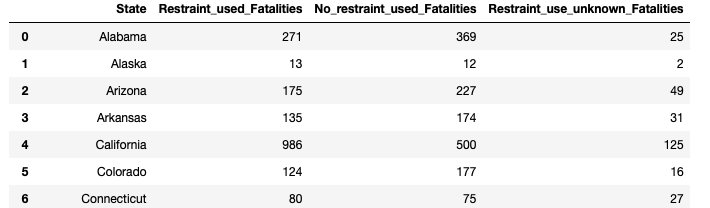
\includegraphics[width=.7\textwidth]{ADOA/Images/fatalhead.png}
    \caption{Échantillon des données}%\hrule
    \label{fig1}
\end{figure*}
 \begin{figure*}[h]
    \centering
    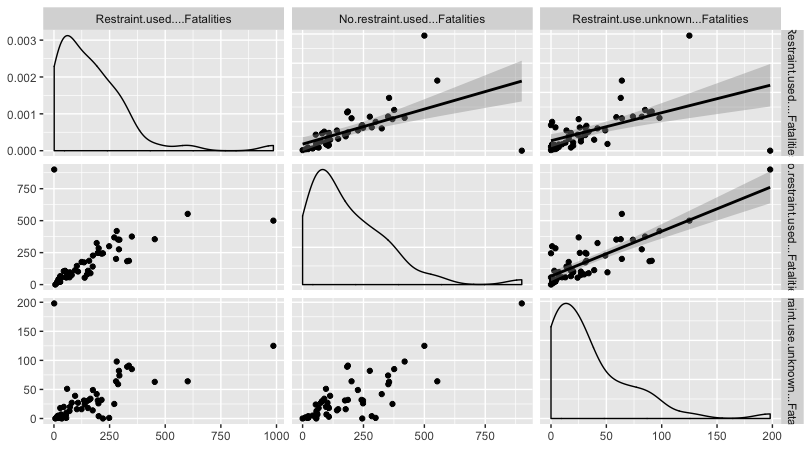
\includegraphics[width=.55\textwidth]{ADOA/Images/Fatal.png}
    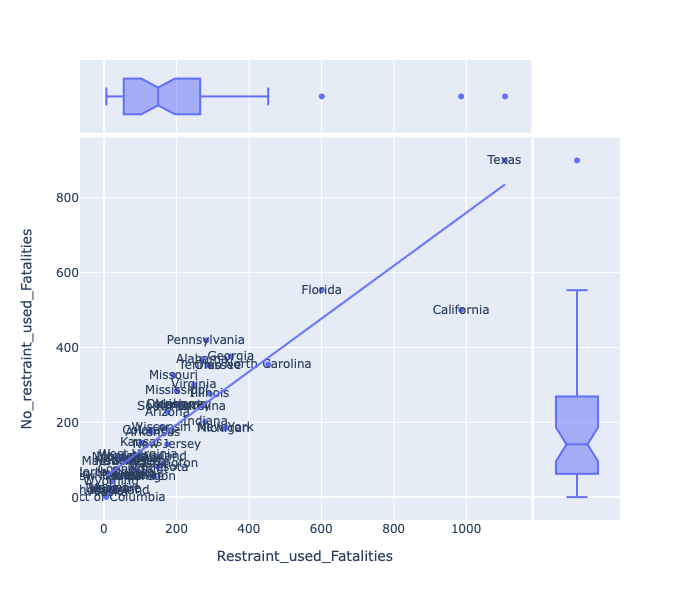
\includegraphics[width=.40\textwidth]{ADOA/Images/Fatal1.png}
    \caption{analyse de 2 composantes}%\hrule
    \label{fig2}
\end{figure*}
 Pour ce faire, les variables sont normalisées afin d’éviter que celles qui ont des grandes échelles dominent les autres. Le resultat est présenté dans la Figure \ref{fig3}. 

 \begin{figure*}[h]
    \centering
    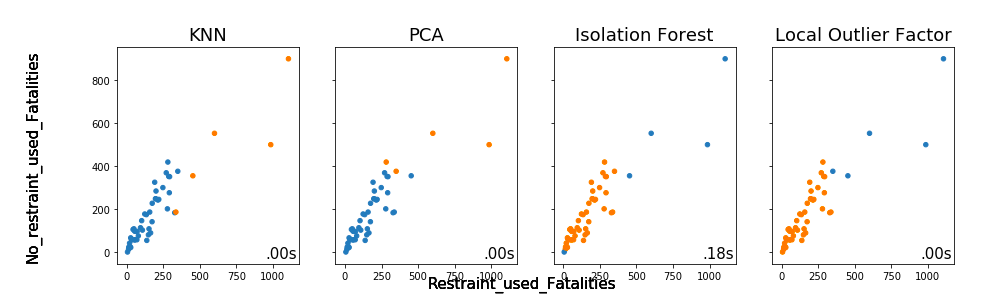
\includegraphics[width=1\textwidth]{ADOA/Images/fatalall.png}
    \caption{Illustration des performences des méthodes: KNN, PCA, Isolation forest and LOF}%\hrule
    \label{fig3}
\end{figure*}
\vspace{2cm}

\textbf{Global cities data set:} 
 C’est une donnée de dimension 68 x 32, les lignes représentent  68 capitales  et les colonnes représentent les caractéristiques  des ces capitales telles que pays, continent, population totale etc.   Il s’agit là d’une détection des valeurs aberrantes non supervisée car on ne connait pas les capitales qui ont des caractéristiques différentes des autres. L’objectif est de repérer les capitales qui ont des particularités différentes par rapport à certaines variables. Les variables suivantes “ Life.Expectancy.in.Years..Male., Life.Expectancy.in.Years..Female. ,Life.Expectancy, Air.Quality., City.Population..millions., Metro.Population..millions, City.Area..km2., Metro.Area..km2.“ ont été extraites puis normalisée avant de les passer aux algorithmes. Le Figure …. Montre les résultats obtenues.
\begin{figure*}[h]
    \centering
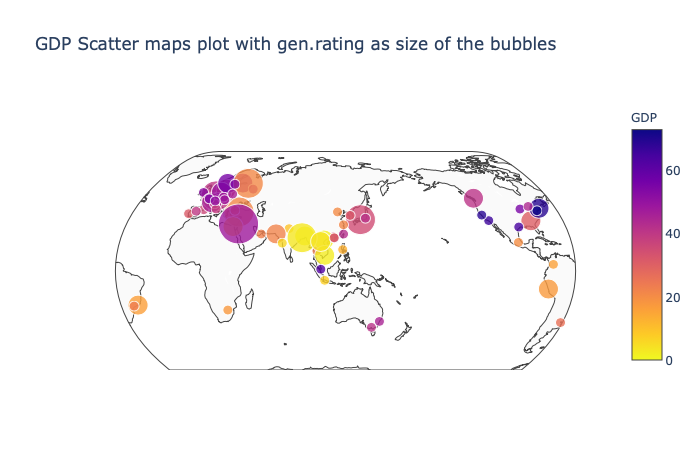
\includegraphics[width=1\textwidth]{ADOA/Images/Glob.png}
    \caption{Global}%\hrule
    \label{fig3}
\end{figure*}

%Perhaps an image (see Figure~\ref{fig:Cities}?
%\begin{figure*}[t]
   % \centering
   % 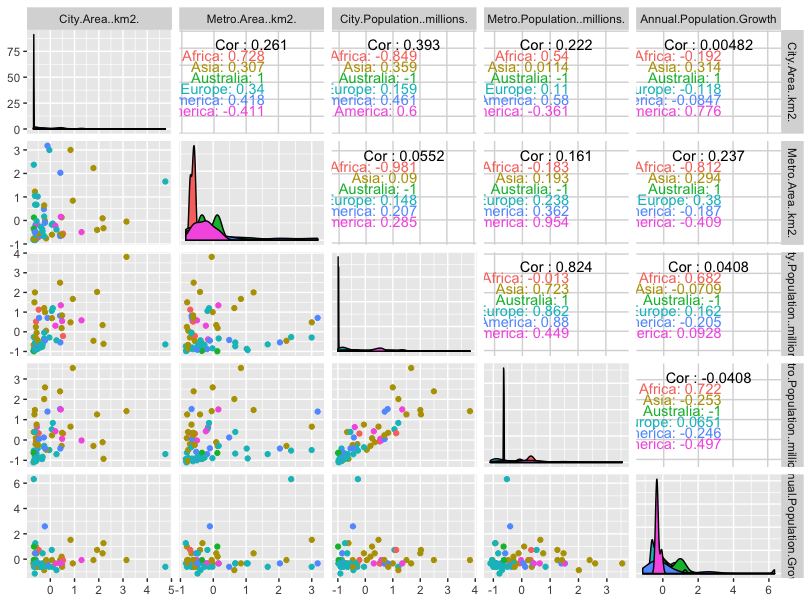
\includegraphics[width=\textwidth]{ADOA/Images/Corr1.png}
   % 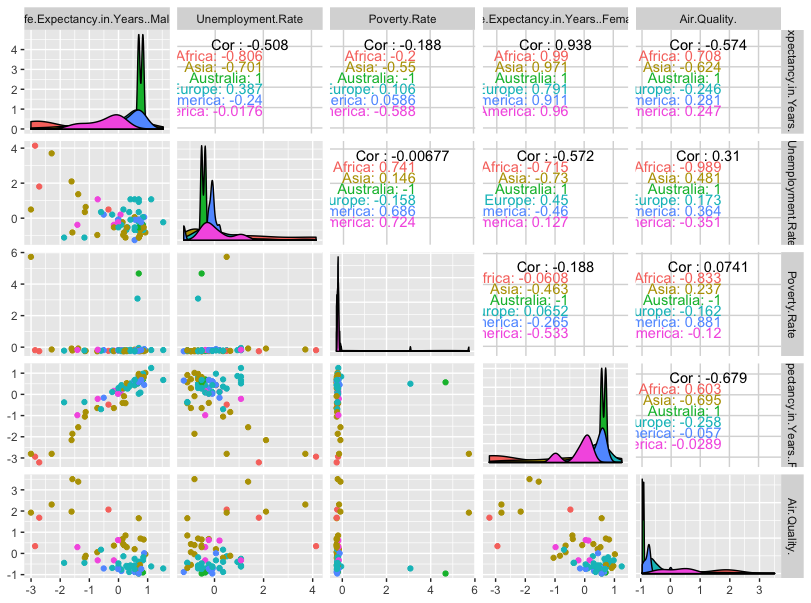
\includegraphics[width=\textwidth]{ADOA/Images/Corr2.png}
   % \caption{.}\hrule
   % \label{fig:Citiesbb}
%\end{figure*}
\begin{figure*}[t]
    \centering
    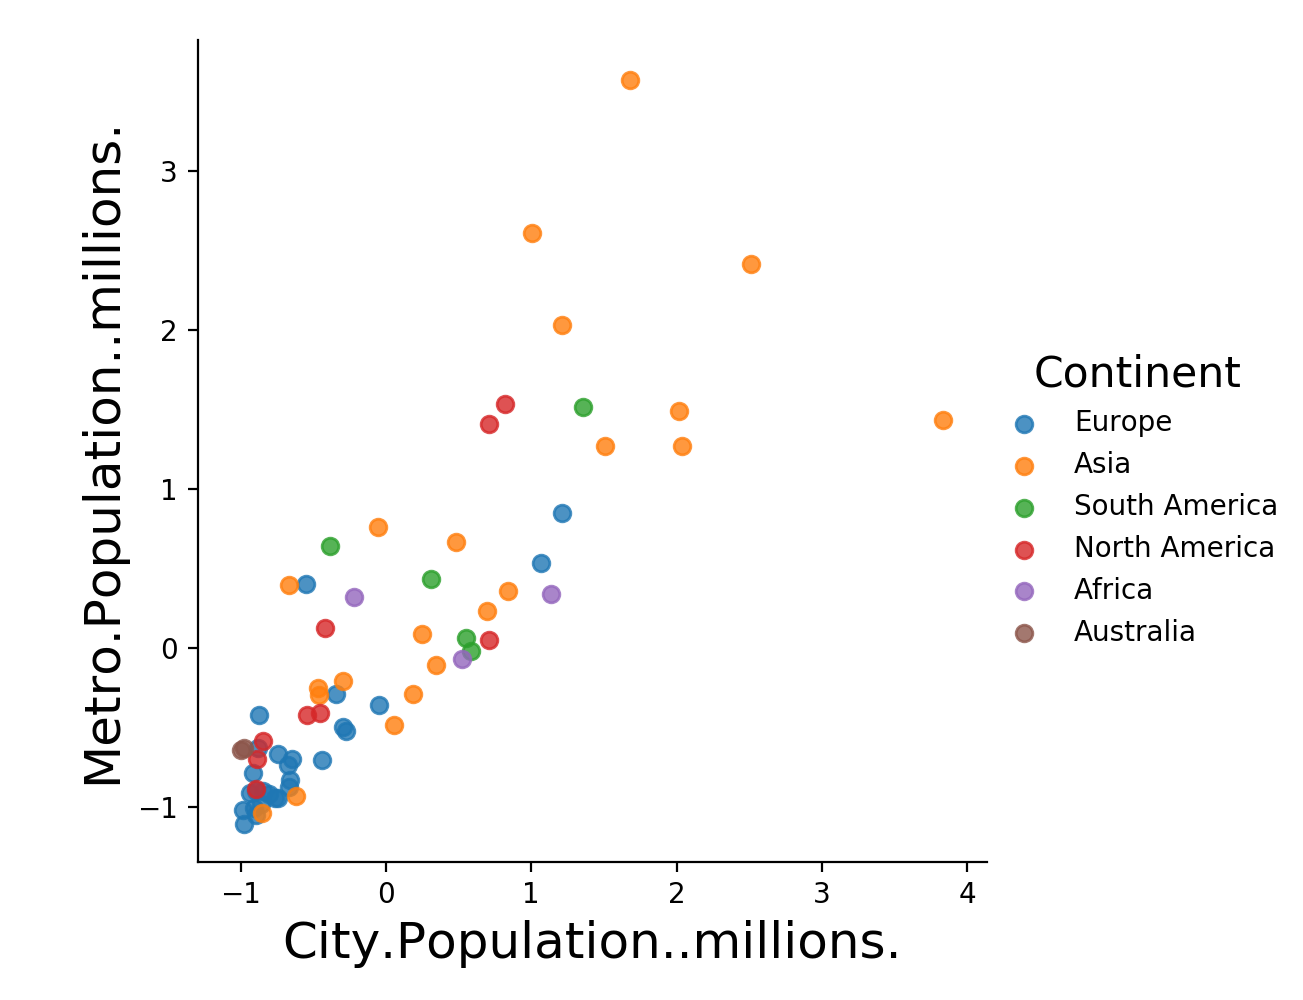
\includegraphics[width=.40\textwidth]{ADOA/Images/CityPopu.png}
    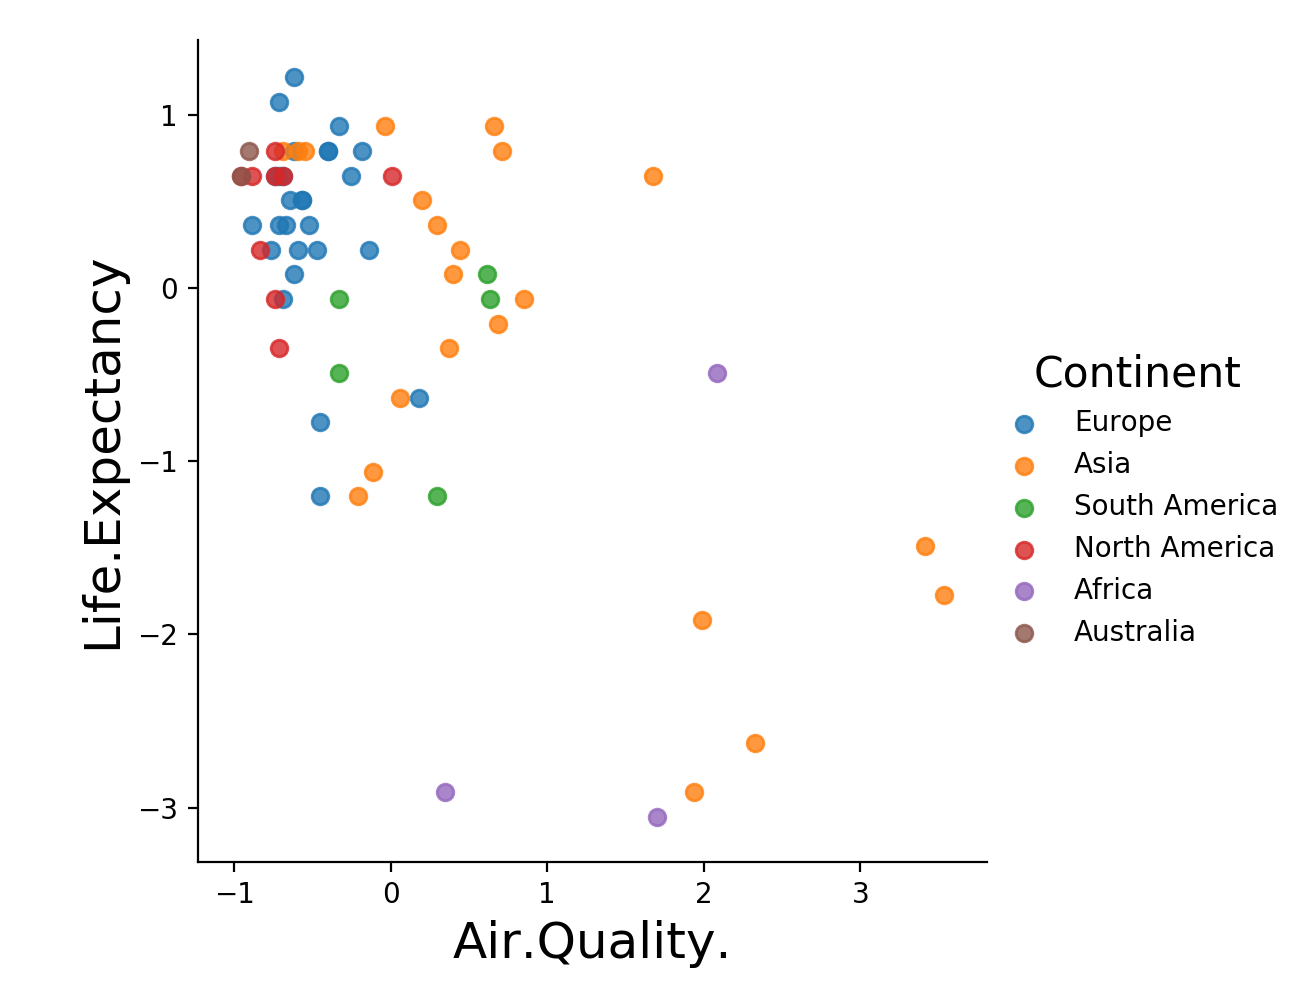
\includegraphics[width=.4\textwidth]{ADOA/Images/AirquaLifeExp.png}
    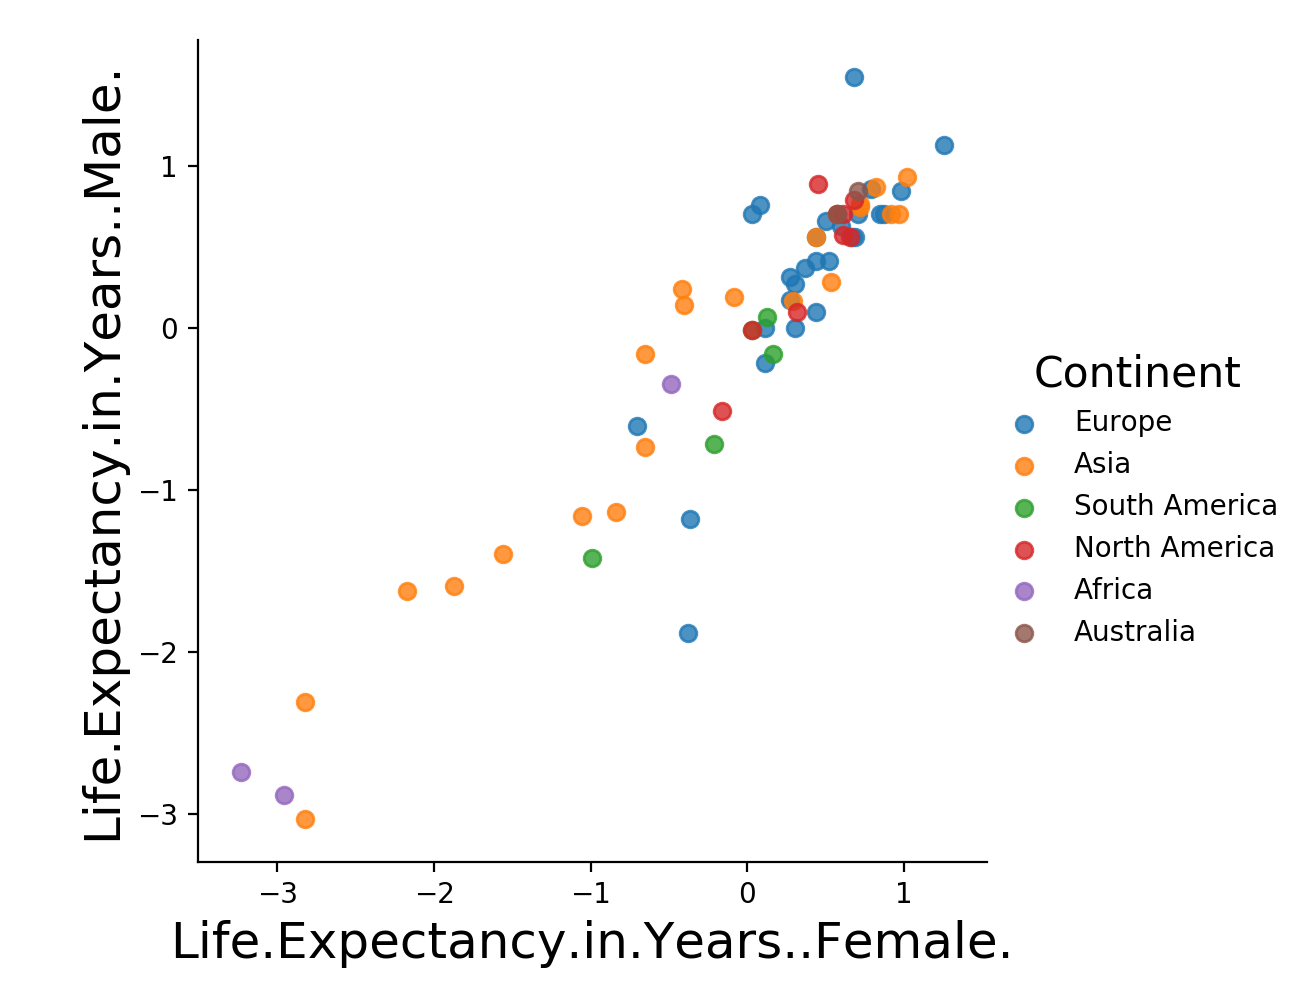
\includegraphics[width=.4\textwidth]{ADOA/Images/LifeExpMaleFemale.png} %
    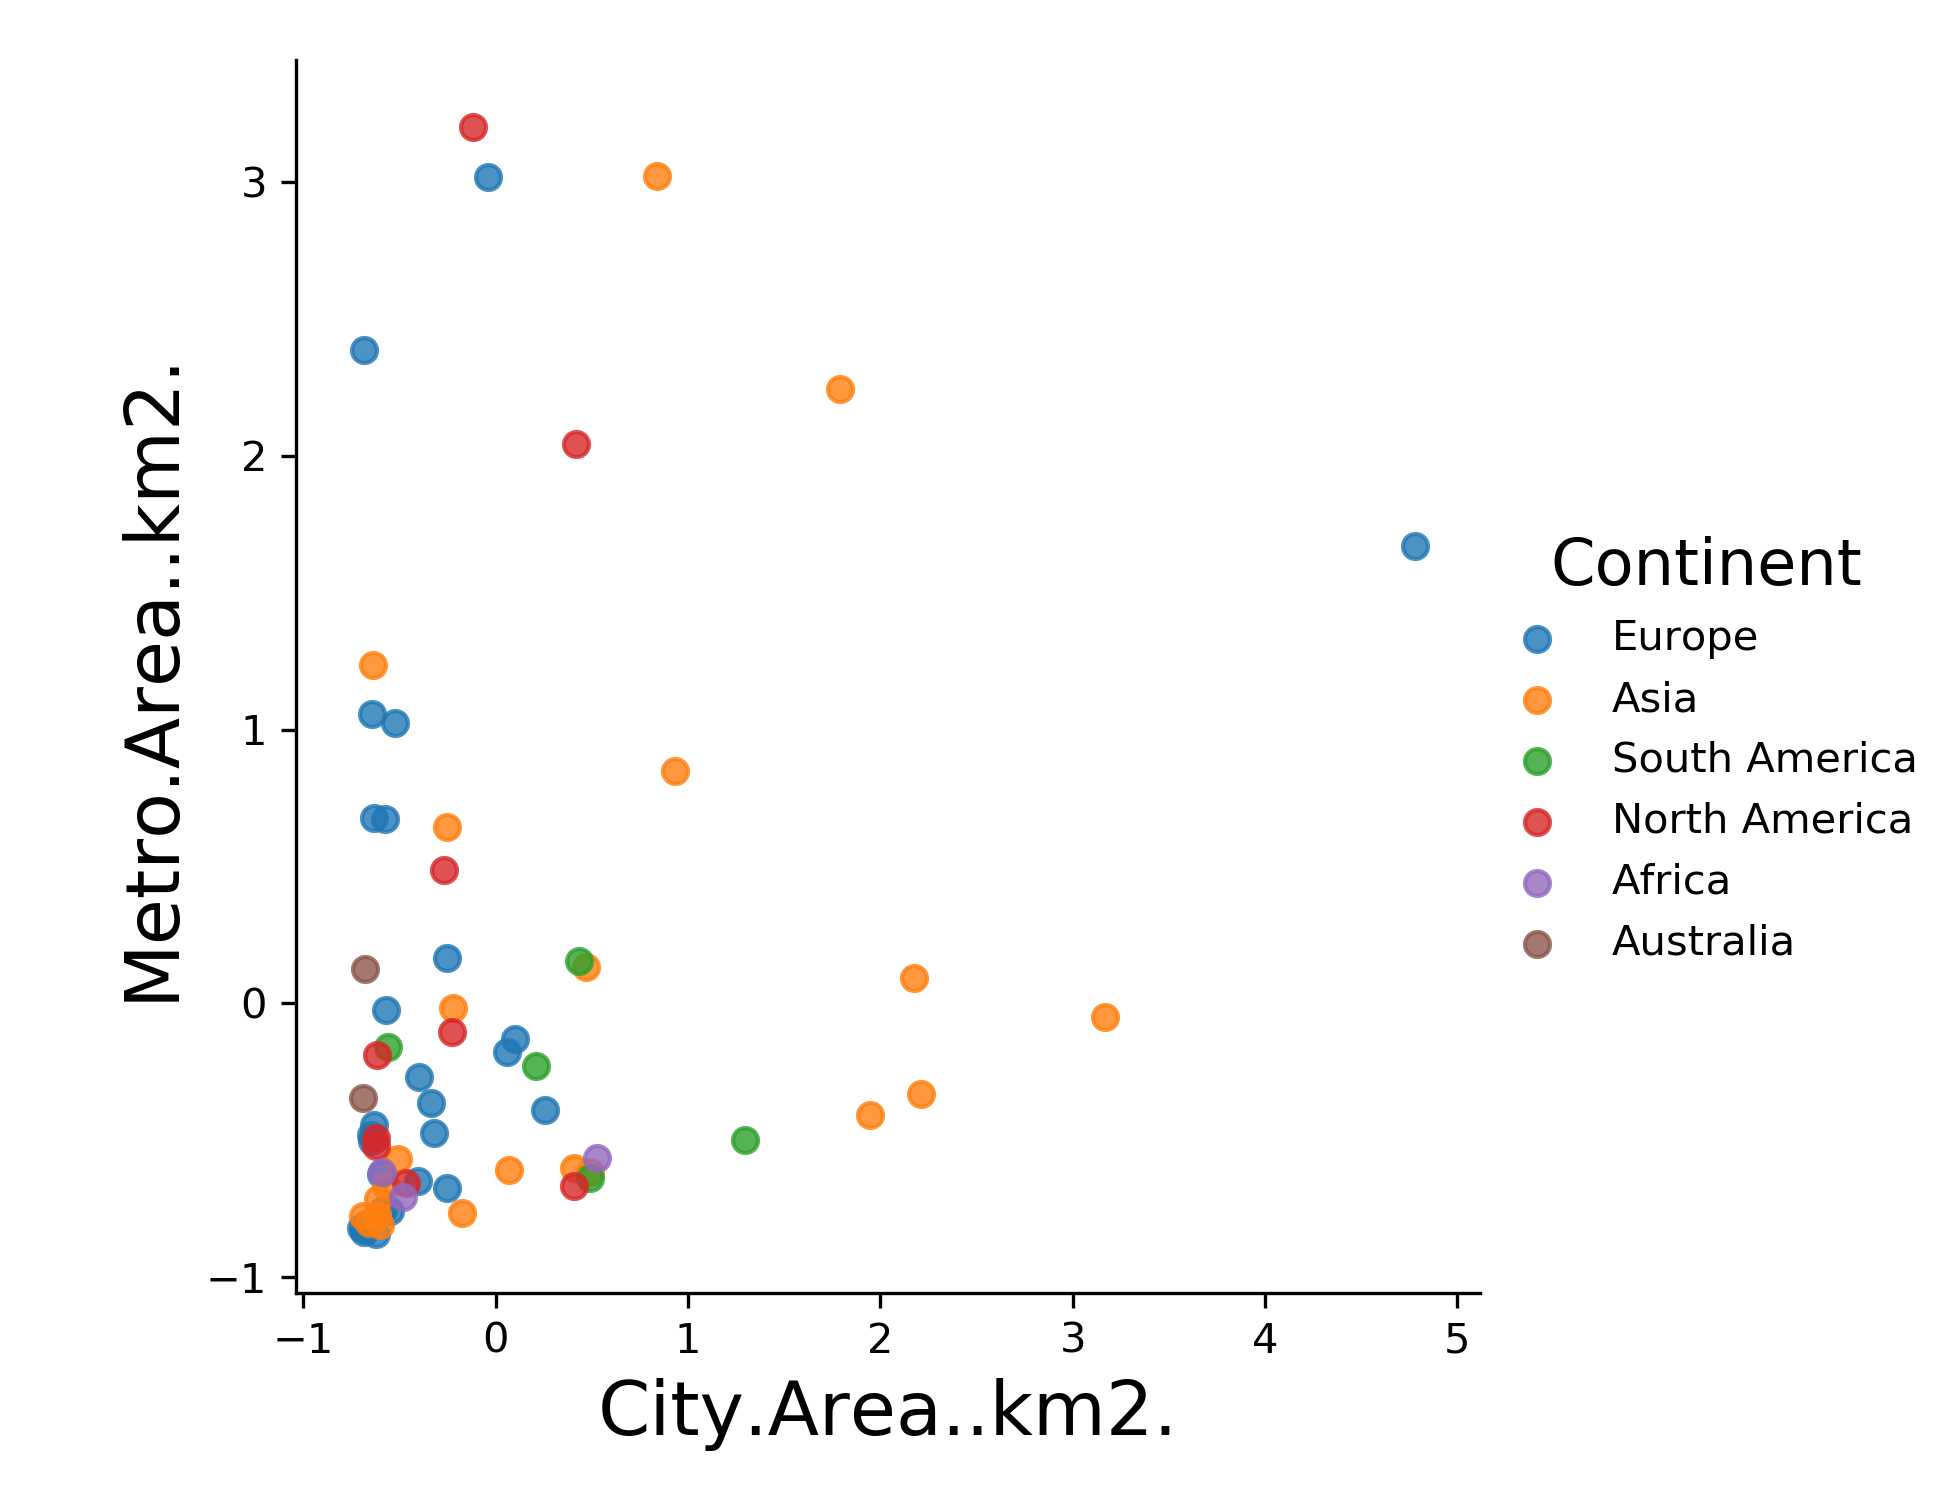
\includegraphics[width=.4\textwidth]{ADOA/Images/CityAreaMetro.png} 
    \caption{.}\hrule
    \label{fig:Citiesb}
\end{figure*}
\begin{figure*}[t]
    \centering
    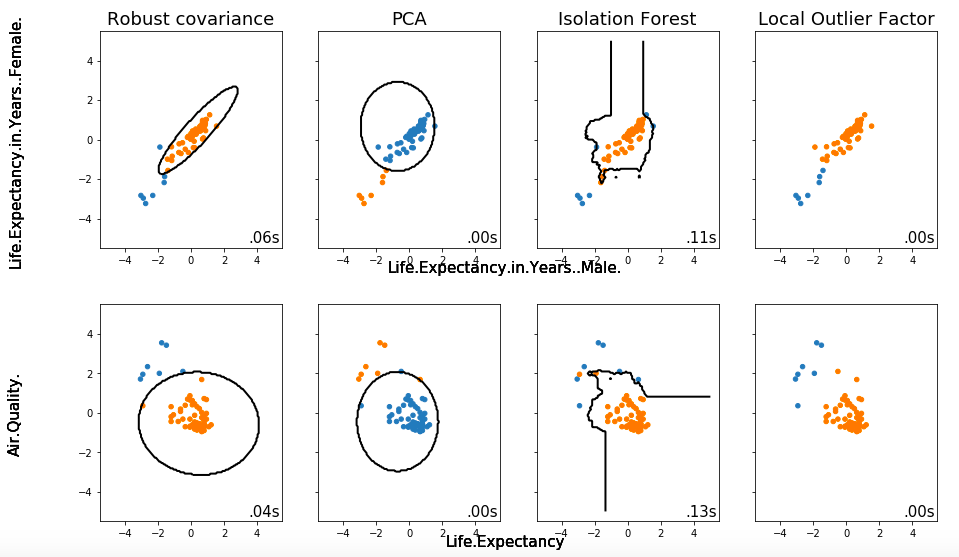
\includegraphics[width=\textwidth]{ADOA/Images/Allcomp1.png}
   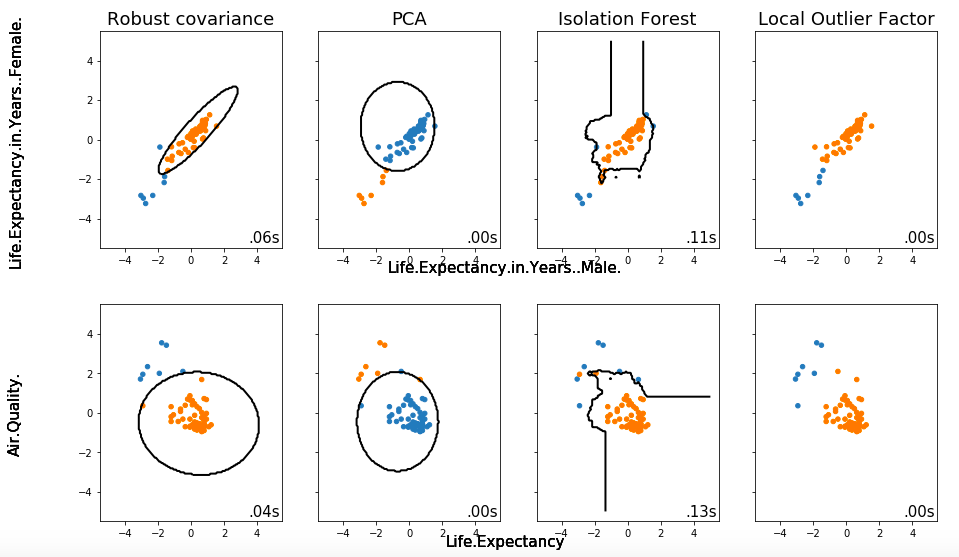
\includegraphics[width=\textwidth]{ADOA/Images/Allcomp1.png}

    \caption{.}\hrule
    \label{fig:Cities}
\end{figure*}
\subsection{Contrôle de qualité}
\subsection{Finance}

%Les occupants d'autres types de véhicules - camions lourds, motos et autobus - sont exclus, de même que les autres types de décès liés aux routes, tels que les décès de piétons. Par conséquent, les accidents mortels représentés ici sont inférieurs à ceux du tableau 2-1. Les pourcentages peuvent ne pas correspondre aux totaux en raison de l'arrondissement.

